\documentclass[border=2pt]{standalone}
\usepackage{tikz}
\usetikzlibrary{arrows.meta,shapes.geometric,topaths}

\begin{document}
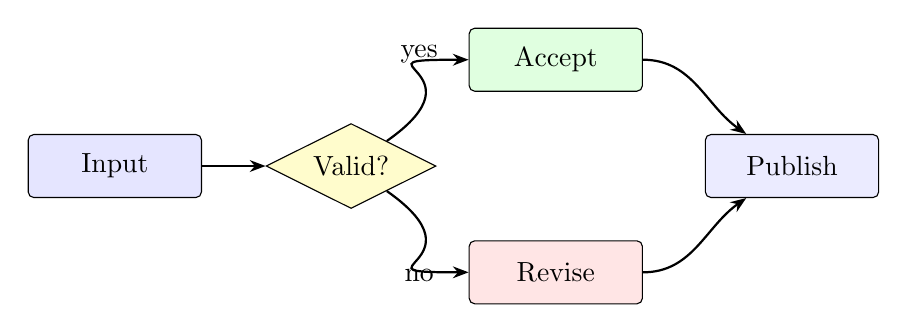
\begin{tikzpicture}[
  process/.style={draw,rounded corners=2pt,minimum width=22mm,minimum height=8mm,align=center},
  decision/.style={draw,diamond,aspect=2,minimum width=20mm,minimum height=10mm,align=center},
  route/.style={-{Stealth[length=2mm]},thick}
]
  \node[process,fill=blue!10] (input) at (0,0) {Input};
  \node[decision,fill=yellow!20] (check) at (3,0) {Valid?};
  \node[process,fill=green!12] (accept) at (5.6,1.35) {Accept};
  \node[process,fill=red!10] (revise) at (5.6,-1.35) {Revise};
  \node[process,fill=blue!8] (publish) at (8.6,0) {Publish};

  \path[route]
    (input) edge (check)
    (check) edge[out=35,in=180,min distance=16mm] node[above] {yes} (accept)
    (check) edge[out=-35,in=180,min distance=16mm] node[below] {no} (revise)
    (accept) edge[out=0,in=145,max distance=8mm] (publish)
    (revise) edge[out=0,in=-145,max distance=8mm] (publish);
\end{tikzpicture}
\end{document}
